\documentclass[border=8pt]{standalone}
\usepackage[T1]{fontenc}
\usepackage{amsmath}
\usepackage{tikz}
\usetikzlibrary{positioning,arrows.meta,calc}
\begin{document}
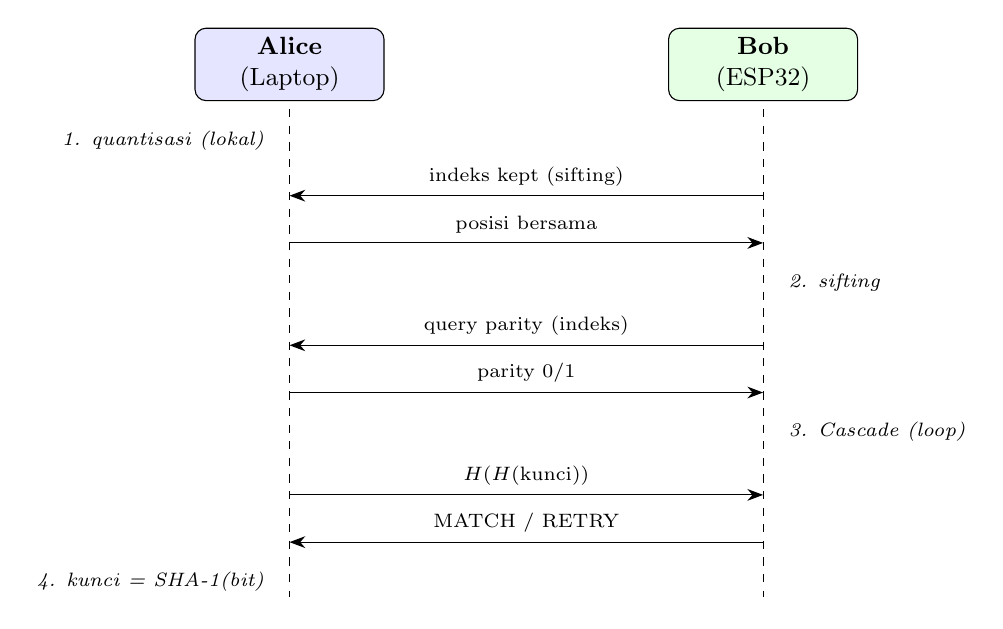
\begin{tikzpicture}[
  node distance=0.45cm and 3.6cm,
  box/.style={draw,rounded corners,align=center,minimum width=2.4cm,minimum height=0.8cm,font=\small},
  msg/.style={-{Stealth[length=2mm]},font=\scriptsize},
]
\node[box,fill=blue!10] (a) {\textbf{Alice}\\(Laptop)};
\node[box,fill=green!10,right=of a] (b) {\textbf{Bob}\\(ESP32)};
\coordinate (a0) at ($(a.south)+(0,-0.1)$);
\coordinate (b0) at ($(b.south)+(0,-0.1)$);
\draw[dashed] (a0) -- ($(a0)+(0,-6.2)$);
\draw[dashed] (b0) -- ($(b0)+(0,-6.2)$);
\node[font=\scriptsize\itshape,anchor=east] at ($(a0)+(-0.2,-0.4)$) {1. quantisasi (lokal)};
\draw[msg] ($(b0)+(0,-1.1)$) -- node[above]{indeks kept (sifting)} ($(a0)+(0,-1.1)$);
\draw[msg] ($(a0)+(0,-1.7)$) -- node[above]{posisi bersama} ($(b0)+(0,-1.7)$);
\node[font=\scriptsize\itshape,anchor=west] at ($(b0)+(0.2,-2.2)$) {2. sifting};
\draw[msg] ($(b0)+(0,-3.0)$) -- node[above]{query parity (indeks)} ($(a0)+(0,-3.0)$);
\draw[msg] ($(a0)+(0,-3.6)$) -- node[above]{parity 0/1} ($(b0)+(0,-3.6)$);
\node[font=\scriptsize\itshape,anchor=west] at ($(b0)+(0.2,-4.1)$) {3. Cascade (loop)};
\draw[msg] ($(a0)+(0,-4.9)$) -- node[above]{$H(H(\text{kunci}))$} ($(b0)+(0,-4.9)$);
\draw[msg] ($(b0)+(0,-5.5)$) -- node[above]{MATCH / RETRY} ($(a0)+(0,-5.5)$);
\node[font=\scriptsize\itshape,anchor=east] at ($(a0)+(-0.2,-6.0)$) {4. kunci = SHA-1(bit)};
\end{tikzpicture}
\end{document}
